\section{Intelligenze Artificiale}
\subsection{Introduzione alla Materia}
L'intelligenza artificiale ha origine negli anni 40 con la cibernetica, ovvero costruire modelli meccanici in grado di simulare il comportamento adattivo di sistemi naturali. L’intuizione principale della cibernetica è stato quello di proporre una prospettiva unificata allo studio di organismi biologici e macchine.

"L'intelligenza artificiale è una branca dell’informatica che studia i fondamenti teorici, le metodologie e le tecniche che consentono la progettazione di sistemi hardware e software capaci di fornire a un calcolatore prestazioni che, a un osservatore comune, sembrerebbero essere di pertinenza esclusiva dell’intelligenza umana." (Somalvico, 2003)

\begin{figure}[h]
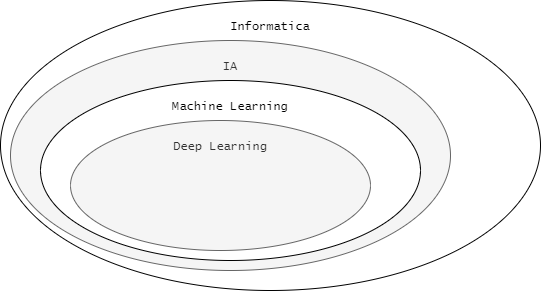
\includegraphics[scale=0.5]{IA e Informatica}
\centering
\end{figure}

Come illustrato nel diagramma, l'intelligenza artificiale è un sottoinsieme dell'informatica ed è bene sottolineare che al suo interno si incontrano diverse discipline:
\begin{itemize}
    \item Ingegneristica: costruire macchine capaci di svolgere compiti intelligenti integrando componenti diverse.
    \item Psicologica: costruire macchine capaci di esprimere le caratteristiche essenziali dell’attività cognitiva umana spiegando i rapporti tra pensiero e fisicità dell’uomo.
\end{itemize}

\subsection{Approcci}

Esistono diversi tipi di approccio alla materia:

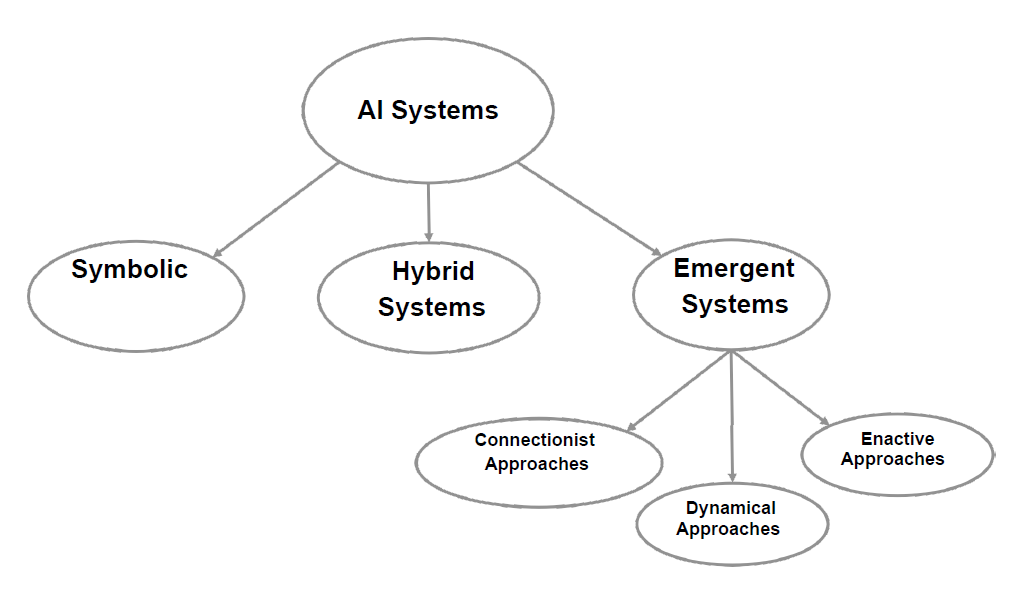
\includegraphics[scale=0.4]{IA Approcci}

Gli approcci principali sono:
\begin{itemize}
    \item Emergentista (Emergent System): tutti i sistemi facente parte di questo approccio sono basati sull'apprendimento, quindi si nutrono di dati.
    \begin{itemize}
        \item Connectionist Approaches: un approccio che si è sviluppato dai tentativi di capire come funziona il cervello umano a livello neurale e, in particolare, come le persone imparano e ricordano.
        \item Dynamical Approaches: un approccio applicato allo studio dei sistemi automatici.
        \item Enactive Approaches: è focalizzato sulle azioni mirate e sulle interazioni dinamiche reciproche con l'ambiente riunendo mente/cervello, mente/corpo e corpo/ambiente. Ad esempio, quello che una macchina, un robot, ha con l'ambiente circostante utilizzando i sensori.
    \end{itemize}
    \item Simbolico (Symbolic System): tutti i sistemi facente parte di questo approccio applicano una logica "top down", vengono implementate delle reti semantiche di concetti e predicati.
    \item Ibrido (Hybride System): sistemi ibridi
\end{itemize}

\subsection{Intelligenza Artificiale Forte e Debole}
Con il termine "IA forte" ci si riferisce a quella teoria che afferma che la macchina che agisce in modo “intelligente” possiede una “mente” e una “coscienza”, e quindi “pensa", esattamente nel modo in cui accade agli esseri umani (o ad altri animali).

Con il termine "IA debole" ci si riferisce alla tesi sostenuta dalla comunità scientifica moderna, ovvero che le simulazioni al calcolatore dei processi o capacità mentali non vanno confusi con la loro riproduzione.

\subsection{Obiettivi}
L'obiettivo dell'IA è quello di rendere le macchine intelligenti, in grado di replicare come l'essere umano agisce, o reagisce, ad uno stimolo sulla base di ciò che ha appreso fino a quel momento. 

Di fatto l'essere umano apprende a seconda delle esperienze maturate, positive o negative che siano.
Questa conoscenza esplicita viene utilizzata per ragionare e \textbf{inferire} nuova conoscenza, ad esempio, sappiamo che "i gatti miagolano", che Tom è un gatto e possiamo inferire che Tom miagola.

Bisogna tenere a mente però che l'essere umano, cosi come i sistemi intelligenti, sono sempre in possesso di conoscenza parziale, incerta o errata. Questo è un problema soprattutto per i sistemi intelligenti perché, a differenza degli esseri umani, il \textbf{ragionamento è monotòno}, quindi l'aggiunta di nuove asserzioni o regole alla base di conoscenza non può invalidare teoremi precedentemente dimostrati, ma solo aggiungerne di nuovi.

Il ragionamento, le inferenze, che l'essere umano fa è spesso non monotòno: si fanno inferenze tentative, anche in mancanza di informazioni complete e, a fronte di nuove conoscenza, si rivedono le inferenze o le assunzioni precedentemente fatte.

\subsection{Laboratorio: Introduzione a Prolog}
Il Prolog è un linguaggio di programmazione che adotta il paradigma di programmazione logica. E' un interprete che permette di dimostrare dei fatti a partire da un dominio di conoscenza costituito da \textbf{fatti} e \textbf{clausole}.
Bisogna osservare alcune informazioni importanti prima di proseguire: 
\begin{itemize}
    \item I fatti terminano sempre con il "."
    \item Le costanti hanno la prima lettera minuscola
    \item Le variabili hanno la prima lettera maiuscola
    \item Per uscire dall'editor Ctrl+D o \textit{?- halt.}
    \item Per utilizzare la modalità debug \textit{?-trace.} e per uscire \textit{?-nodebug.}
    \item Includere nuovi file è possibile con il comando \textit{?- consult(fileName).} oppure \textit{?- ['nomeFile'].}
\end{itemize}

Il \textbf{fatto} è un insieme di informazioni esplicite relative al mio dominio, ad esempio "Tom è un gatto", la sintassi è la seguente:
\begin{tcblisting}{breakable,listing only,
  listing options={language=Prolog,aboveskip=0pt,belowskip=0pt},
  size=fbox,boxrule=0pt,frame hidden,arc=0pt}
gatto(tom).
\end{tcblisting}
Un fatto è costituito da un \textbf{predicato}, che è una funzione senza argomento, nel nostro esempio è "gatto" e da una costante, ovvero "tom".

Una \textbf{regola} di inferenza è uno schema formale che si applica nell'eseguire un'inferenza, una \textbf{clausola} è un insieme finiti di fatti e regole.

Di seguito un semplice esempio di programma che definisce fatti e regole:
\begin{tcblisting}{breakable,listing only,
  listing options={language=Prolog,aboveskip=0pt,belowskip=0pt},
  size=fbox,boxrule=0pt,frame hidden,arc=0pt}
% Regola: "tutti i gatti sono felini"
felino(X):-gatto(X).

% Regola: "gli uccelli volano"
vola(X):-uccelli(X)
\end{tcblisting}

Per utilizzare il linguaggio matematico una regola può essere scritta nel seguente modo:
\begin{displaymath}
\forall X : gatto(X) = true => felino(X) = true
\end{displaymath}

Di seguito un semplice esempio di programma che definisce fatti e regole:
\begin{tcblisting}{breakable,listing only,
  listing options={language=Prolog,aboveskip=0pt,belowskip=0pt},
  size=fbox,boxrule=0pt,frame hidden,arc=0pt}
% Fatti
gatto(tom).
gatto(fred).
tigre(mike).
vivo(tom).

% Regole
felino(X):-gatto(X).
felino(X):-tigre(X).

% Regola: "X miagola se e' un gatto AND e' vivo"
miagola(X):-gatto(X),vivo(X).
\end{tcblisting}

Da interprete possiamo effettuare un test veloce, come primo passaggio però dovremmo importare il file contenente i fatti e le regole appena mostrate:

\begin{tcblisting}{breakable,listing only,
  listing options={language=Prolog,aboveskip=0pt,belowskip=0pt},
  size=fbox,boxrule=0pt,frame hidden,arc=0pt,colback=lightgray}
?- ['Esercizi/lezione1.pl'].
true.
?- gatto(Chi).
Chi = tom ;
Chi = fred.
?- felino(tom). % deduzione
true.
?- gatto(mike). 
false.
\end{tcblisting}

\subsection{Laboratorio: Congiunzione e Disgiunzione Logica}
Come accennato in precedenza la congiunzione, l'and booleano, può essere implementata utilizzando la virgola ",", per quanto riguarda la disgiunzione, quindi l'or booleano, sarà sufficiente definire più clausole.

Di seguito un esempio che racchiude quanto detto:
\begin{tcblisting}{breakable,listing only,
  listing options={language=Prolog,aboveskip=0pt,belowskip=0pt},
  size=fbox,boxrule=0pt,frame hidden,arc=0pt}
% fatti: genitore e figli
genitore(paolo,mario).
genitore(anna,mario).
genitore(paolo,luisa).
genitore(anna,luisa).
% paolo e' nonno di chiara
genitore(mario,chiara). 

 % paolo e' padre di marco, marco non ha una madre
genitore(paolo,marco).
                       
genitore(antonella,chiara).

genitore(mario,alberto).
genitore(francesca,alberto).
genitore(marco,serena).
genitore(serena,fabrizio).
genitore(fabrizio,lorenzo).

% regole
nonno(X,Y):-genitore(X,Z),genitore(Z,Y).

antenato(X,Y):-genitore(X,Y).
antenato(X,Y):-nonno(X,Y).
antenato(X,Y):-genitore(X,Z),antenato(Z,Y).
\end{tcblisting}

Analizzando quanto scritto notiamo che è stata implementata una disgiunzione logica con le regole:
\begin{tcblisting}{breakable,listing only,
  listing options={language=Prolog,aboveskip=0pt,belowskip=0pt},
  size=fbox,boxrule=0pt,frame hidden,arc=0pt}
antenato(X,Y):-genitore(X,Y).
antenato(X,Y):-nonno(X,Y).
\end{tcblisting}
Quanto scritto sta ad indicare che X è un antenato di Y sse X è genitore di Y \textbf{oppure} X è nonno di Y, notare che X e Y sono delle variabili.

Inoltre possiamo pensare di generalizzare utilizzando una regola ricorsiva dove il caso base verifica che che X sia antenato di Y con la regola della genitorialità, mentre invece il caso ricorsivo verifica che X sia genitore di Z \textbf{oppure} che Z sia antenato di Y:
\begin{tcblisting}{breakable,listing only,
  listing options={language=Prolog,aboveskip=0pt,belowskip=0pt},
  size=fbox,boxrule=0pt,frame hidden,arc=0pt}
antenato(X,Y):-genitore(X,Y).
antenato(X,Y):-genitore(X,Z),antenato(Z,Y).
\end{tcblisting}

In ultimo istanza implementiamo la regola \textbf{fratelloGermano} verifica se A e B sono fratelli, dove A è diverso da B:
\begin{tcblisting}{breakable,listing only,
  listing options={language=Prolog,aboveskip=0pt,belowskip=0pt},
  size=fbox,boxrule=0pt,frame hidden,arc=0pt}
fratelloGermano(A,B):-
    % A != B
    A \== B,
    
    % A e B sono fratelli se hanno gli stessi genitori
    genitore(PrimoGenitore,A),
    genitore(SecondoGenitore,A),
    genitore(PrimoGenitore,B),
    genitore(SecondoGenitore,B).
\end{tcblisting}